%  Pt1.tex
% !TeX spellcheck = en_GB
% !TeX root = ProjectRiskManagement.tex

\section{The PUMP Approach to Uncertainty and Underlying Complexity Management}

%Introduction to risk and opportunity, underlying complexity. 

%Challenge of traditional view of risk.
The phrasing ``uncertainty and underlying complexity management'' has been specifically selected as the title of this section to contrast with the risk management title of the course as a whole.
Traditional views of risk management offer a limited scope and an incomplete picture.
Often the focus is event uncertainty reflecting the standard dictionary definition of risk: \textit{a hazard, chance of bad consequences, exposure to mischance} \citep{OED}.
This approach does not address the whole of the uncertainty affecting the project, and in the worst case can lead to failed delivery of project objectives.
The Performance Uncertainty Management Process (PUMP) framework encourages departure from the event-centric approach advocated by best practice, to consider all corporate, operational and planning sources of uncertainty.
This expanded perspective allows the capture of ambiguity uncertainty, inherent variability, systematic uncertainty, as well as event uncertainty.
Utilising the PUMP framework shifts the focus of risk management towards the achievement of opportunity efficiency and risk efficiency, through the vehicle of uncertainty management.

% execution and delivery strategy shaping phase of a project's life cycle
Procedures ensure consistency and quality is maintained throughout repeated applications.
A good procedure is designed to be simple, repeatable and transparent.
However, this cannot be a uniform approach.
Some high complexity, high uncertainty projects require sophisticated, tailored procedures.
The PUMP framework supports this concept through PUMP packs; a set of PUMPs tailored to specific projects and project lifecycle stages.
%Particularly, this paper focusses on PUMPs within the context of the execution and delivery (E\&D) strategy shaping stage.

\subsection{The Project Lifecycle Context}
%Project life cycle introduction.
A traditional four stage view of the asset/change lifecycle is a useful starting point to consider the scope of a project.
The four stages are conceptualize, planning, execution and delivery (E\&D) and Utilization.
As explained, effective uncertainty management requires a macro-view of the entire project to capture the different aspects of uncertainty.
This leads to an elaboration of the lifecycle to incorporate 12 stages, each emphasizing a different management purpose.
There is discussion as to the usefulness of such high clarity in the lifecycle, however it provokes in-depth consideration of all types of uncertainty \citep{Ward1995145}.
Both views are shown in figure \ref{Figure:Project_Lifecycle}.

\begin{figure}[!h]
  \centering
    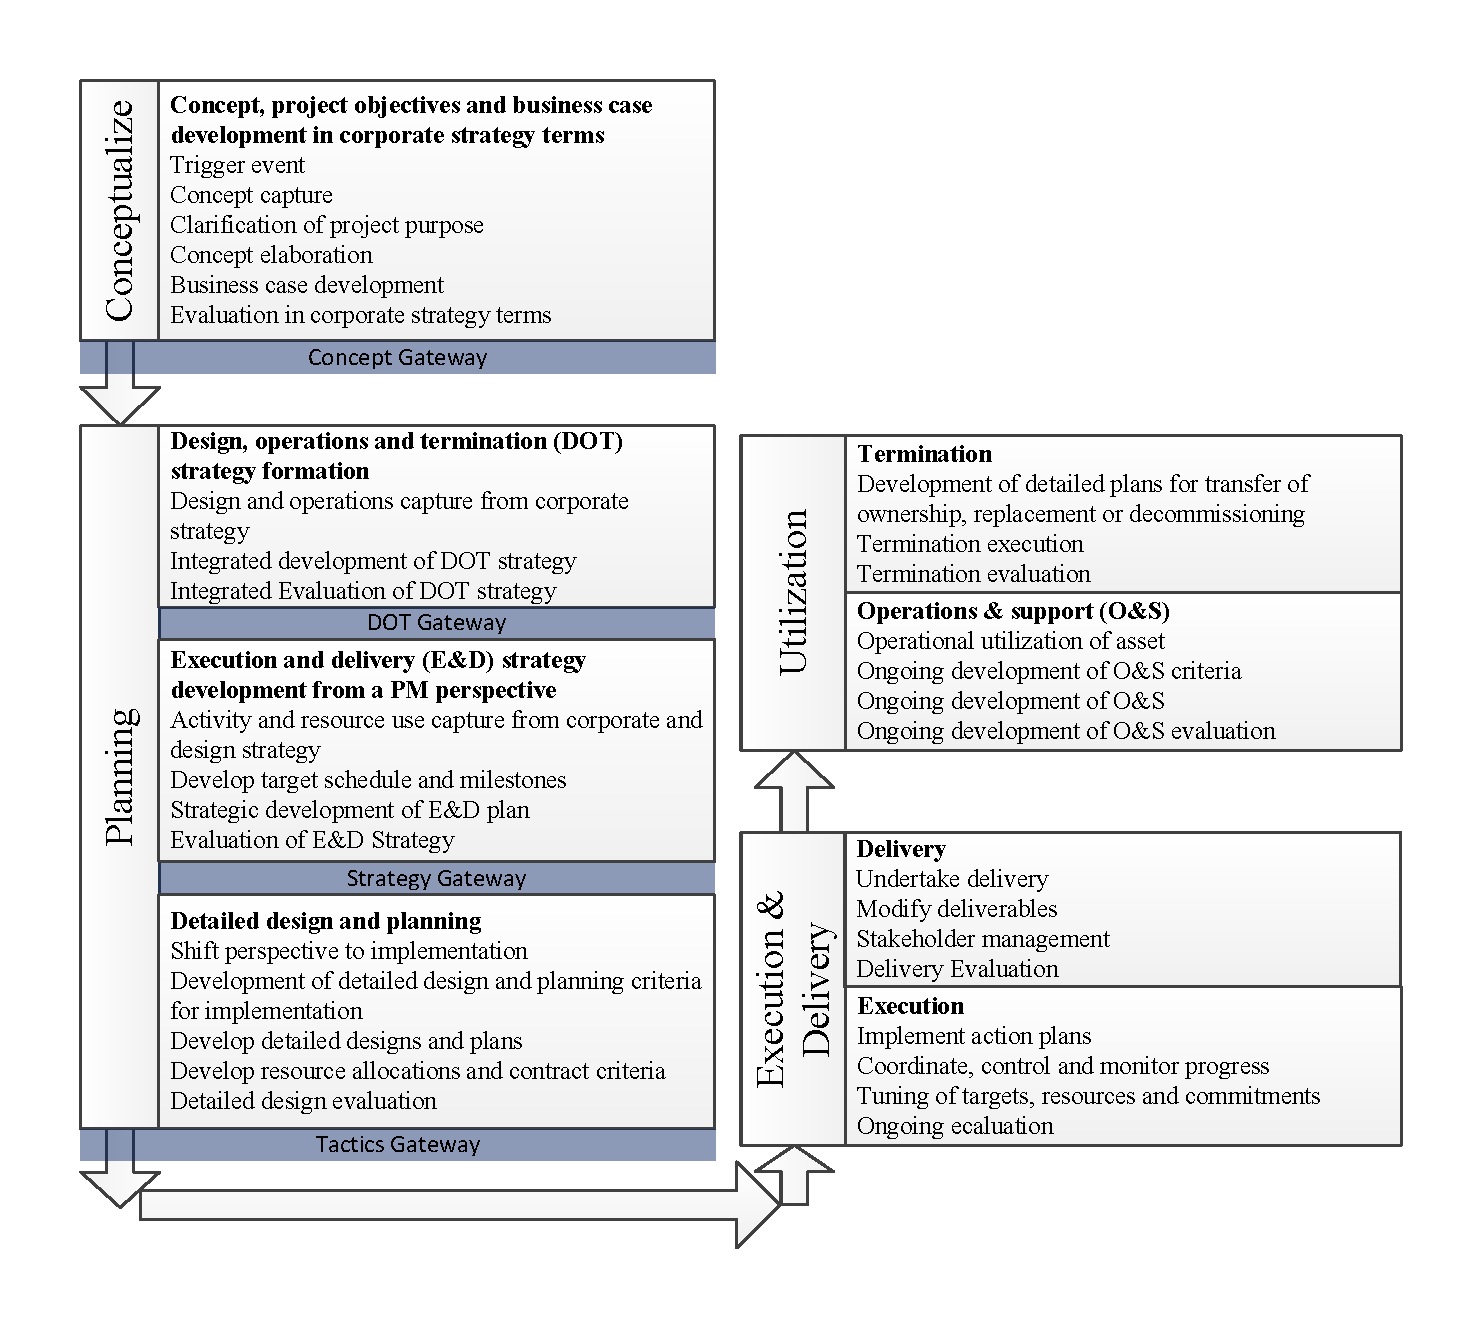
\includegraphics[width = \textwidth]{./Figures/ProjectLifecycleDetailedCurve.png} 
\caption{Twelve-stage asset/change lifecycle - adapted from \cite{chapman}}
\label{Figure:Project_Lifecycle}
\end{figure}

The planning stage of the traditional lifecycle is expanded to three shaping stages and three governance stages.
%The design, operations and termination (DOT) stage aims to derive a strategy for DOT from the corporate strategy developed in the conceptualize stage.
%A basic set of design criteria are built, and the objectives of the project are refined. 
%Integrated evaluation is important to ensure non-viable projects are halted before large expenditure.
The E\&D strategy shaping stage takes a form more familiar in traditional project management.
The activity and resource requirements are derived from the corporate strategy and the design, operations and termination (DOT) strategy. %DOT strategy.
This stage considers aspects of the project execution and asks how the asset/change will be delivered?
Schedule derivation takes place in the E\&D stage, including the reconciliation of corporate expectation and real-world plausibility.
%Again, integrated evaluation is vital to ensuring only viable projects proceed to later more expensive stages of the lifecycle.
Integrated evaluation is vital to ensuring only viable projects proceed to later more expensive stages of the lifecycle.
This paper is concerned with PUMPs tailored to this lifecycle stage.



\subsection{PUMP Overview}
%Explain concisely in your own words what you believe are the key overall features of a PUMP approach to project risk management in the execution and delivery strategy shaping phase of a project’s lifecycle. Compare these features with the PMI PIMBOK approach or any other form of common practice you are familiar with if you find this helpful, but focus on the PUMP approach. Use examples to illustrate your discussion if you wish, but concentrate on concepts and principles. This will be a largely descriptive summary of your interpretation of the lectures and associated reading. It will demonstrate your grasp of the central core of the unit’s material as a whole, and should be approached with a view to demonstrating this understanding..

The PUMP approach was developed through the assimilation of other industrial risk processes, building upon the best practice approaches from project management bodies.
The process was developed by Acres International Management Services for BP and first implemented on the Magnus offshore North Sea project in 1976. 
\citet{SCERT} published the process as SCERT (Synergistic Contingency Evaluation and Review Technique) and the technique has since been used in a variety of high profile projects for BP, National Power and the Highways Agency.
The process has been refined and assimilated into a complete framework suitable for a variety of clarity requirements.


The PUMP process is a seven stage iterative cycle as shown in figure \ref{Figure:Project_Lifecycle}. 
A linear `right first time' approach is not a clarity efficient methodology.
A version of Pareto's principle, sometimes called the 80:20 rule \citep{Pareto1992}, empirically states that 20\% of the issues causes 80\% of the problems. 
The first iteration of the PUMP is a high level sweep to identify the key areas of concern.
Subsequent iterations focus on these issues until a sufficient level of clarity is achieved.
This allows the achievement of clarity efficiency, by minimising time spent on unnecessary detail while achieving the required level of understanding.

\begin{figure}[!h]
  \centering
\subfigure[Flowchart visualisation]{
    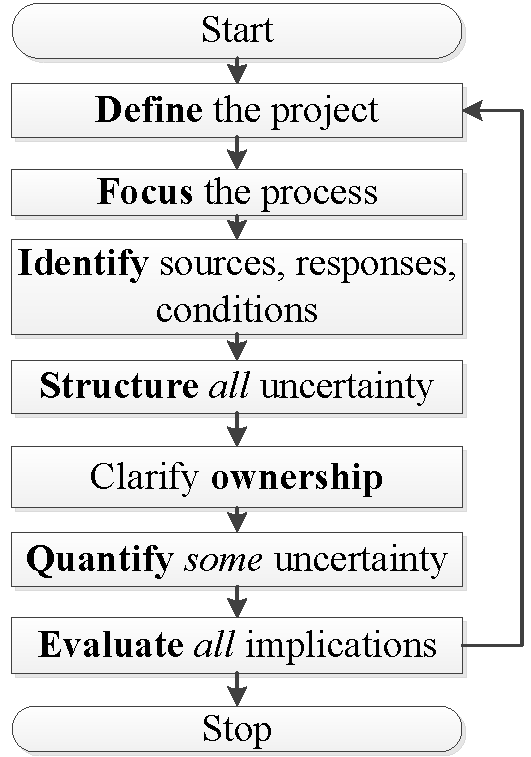
\includegraphics[height = 6cm]{./Figures/PUMPgeneric.png} 
	\label{Figure:GenericPUMP_Flow}
   } \quad
\subfigure[Gantt chart visualisation]{
    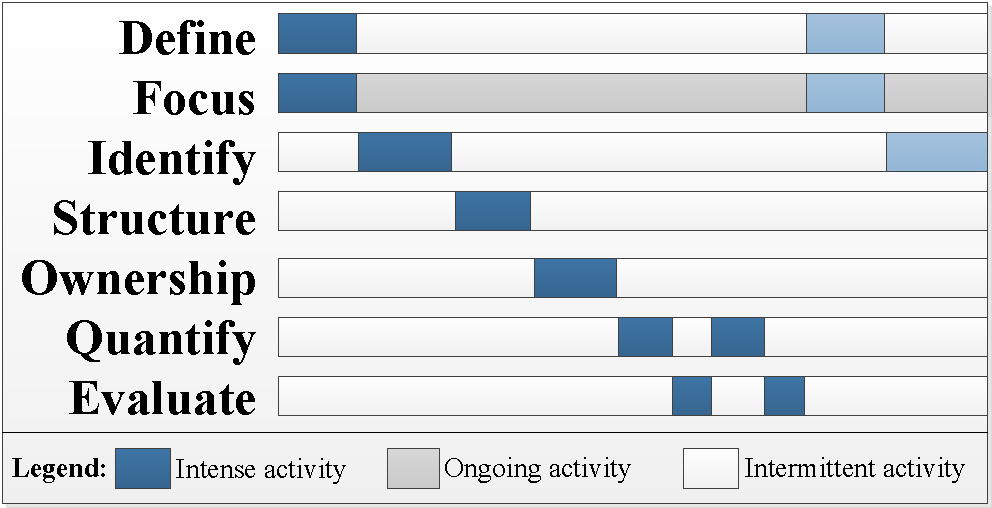
\includegraphics[height = 5cm]{./Figures/PUMPgenericGantt.png} 
	\label{Figure:GenericPUMP_Gantt}
   }
\caption{The generic PUMP process - adapted from \cite{chapman}}
\label{Figure:GenericPUMP_Both}
\end{figure}

The initiating phase of the generic PUMP is the \textbf{define} phase.
This phase defines and develops an understanding of the project as a basis to ask the right questions in subsequent phases.
It features high level context capture and approach development at a strategic level.
There are two key activities in this phase; consolidate and elaborate as shown in figure \ref{Figure:Define}.
A useful framework for adequately addressing these issues is the 7W's: where, who, why, what, whichway, wherewithal, when? 
Using the 7W's to consolidate the existing information, then sub-iterating in order to sufficiently define the project is a useful method to complete this phase.
The phase is complete when the project deliverables are fit for purpose.

The \textbf{focus} phase involves scoping the level of analysis required during the E\&D shaping lifecycle stage.
During this phase, the generic PUMP is tailored to the specific requirements of the project at hand as captured from the corporate context.
This phase is closely coupled with the define phase.
The aim is to achieve clarity efficiency by stating all working assumptions at an early stage.
The phase ends when the scope, strategy and plan for the tailored PUMP process is fit for purpose.

\begin{figure}[!h]
  \centering
\subfigure[Define phase process]{
    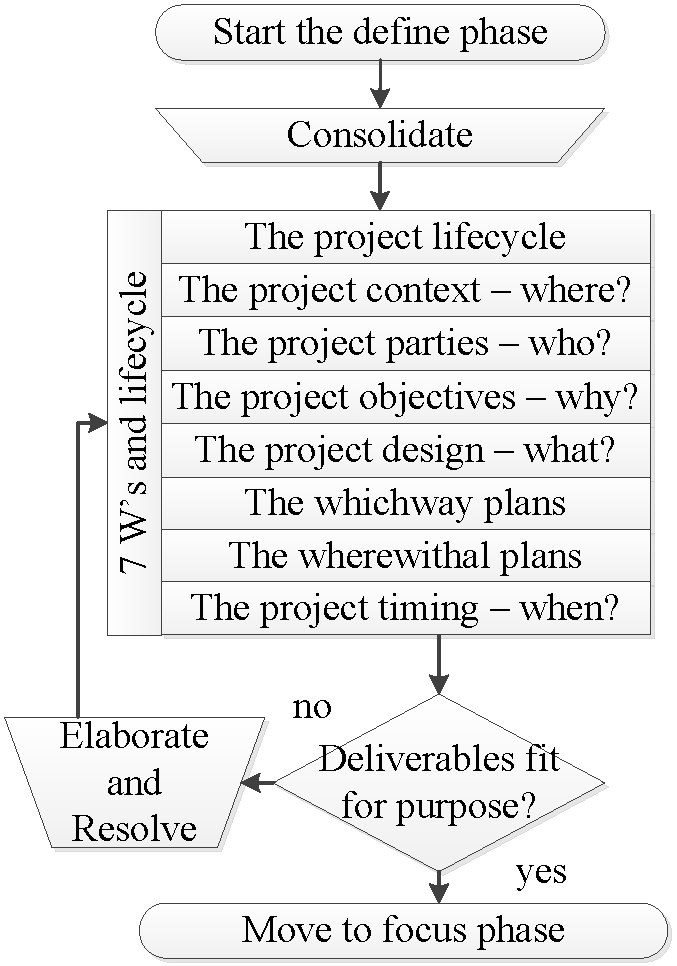
\includegraphics[height = 8cm]{./Figures/Define.png} 
	\label{Figure:Define}
   } \quad
\subfigure[Focus phase process]{
    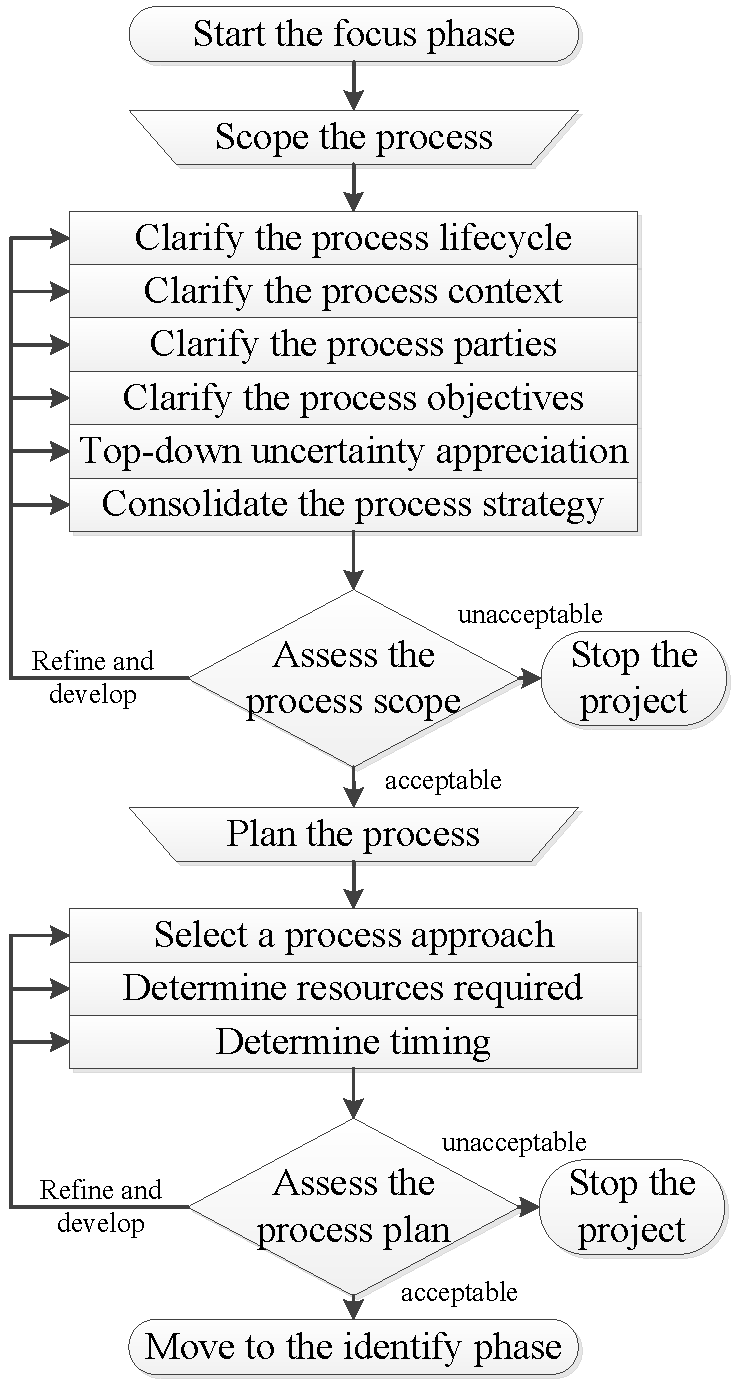
\includegraphics[height = 9.3cm]{./Figures/Focus.png} 
	\label{Figure:Focus}
   }
\caption{Phase process flowcharts - adapted from \cite{chapman}}
\label{Figure:DefineFocus}
\end{figure}

The identification of all sources of uncertainty, relevant response options and conditions is undertaken in the \textbf{identify} phase.
This phase has key distinguishing features that are vital to achieve clarity efficiency and to understand all relevant uncertainty and underlying complexity.
This is considered in detail in section \ref{s:Identify}.

Following the identification of sources of uncertainty, responses and conditions, an understanding of their relative importance is qualitatively established in the \textbf{structure} phase.
This phase contributes to the clarity efficient nature of PUMPs, by maximising the effort expended on issues of perceived importance.
Responses should also be considered, as early identification of powerful general responses means less effort is required to deal with specific responses.
Source-response diagrams, decision tress and influence diagrams are useful tools for this phase.
%\inote{Source-response p215 / faulttree chapman1979/ influencediagram p229}
Failure to deal with underlying complexity, assumptions, interdependencies and detail could endanger the success of the project.
Seemingly small details missed in the structure phase represent systematic uncertainty that could lead to later threats or missed opportunities.
Other key activities are shown in figure \ref{Figure:Structure}.

\begin{figure}[!h]
  \centering
    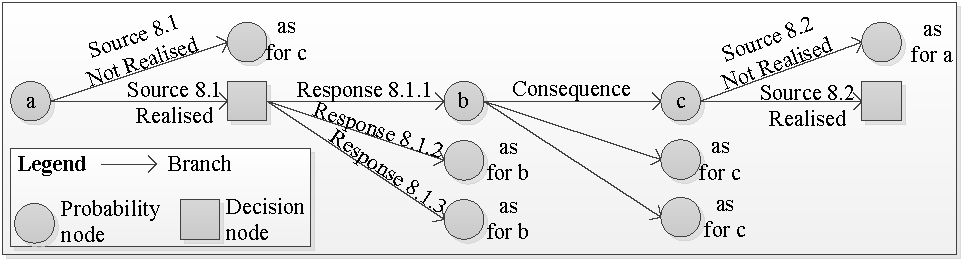
\includegraphics[height = 2.95cm]{./Figures/DecisionTreeChapman79.png} 
\caption{Partial example probability/decision tree - adapted from \cite{SCERT}}
\label{Figure:Decisiontree}
\end{figure}

\begin{figure}[!h]
  \centering
    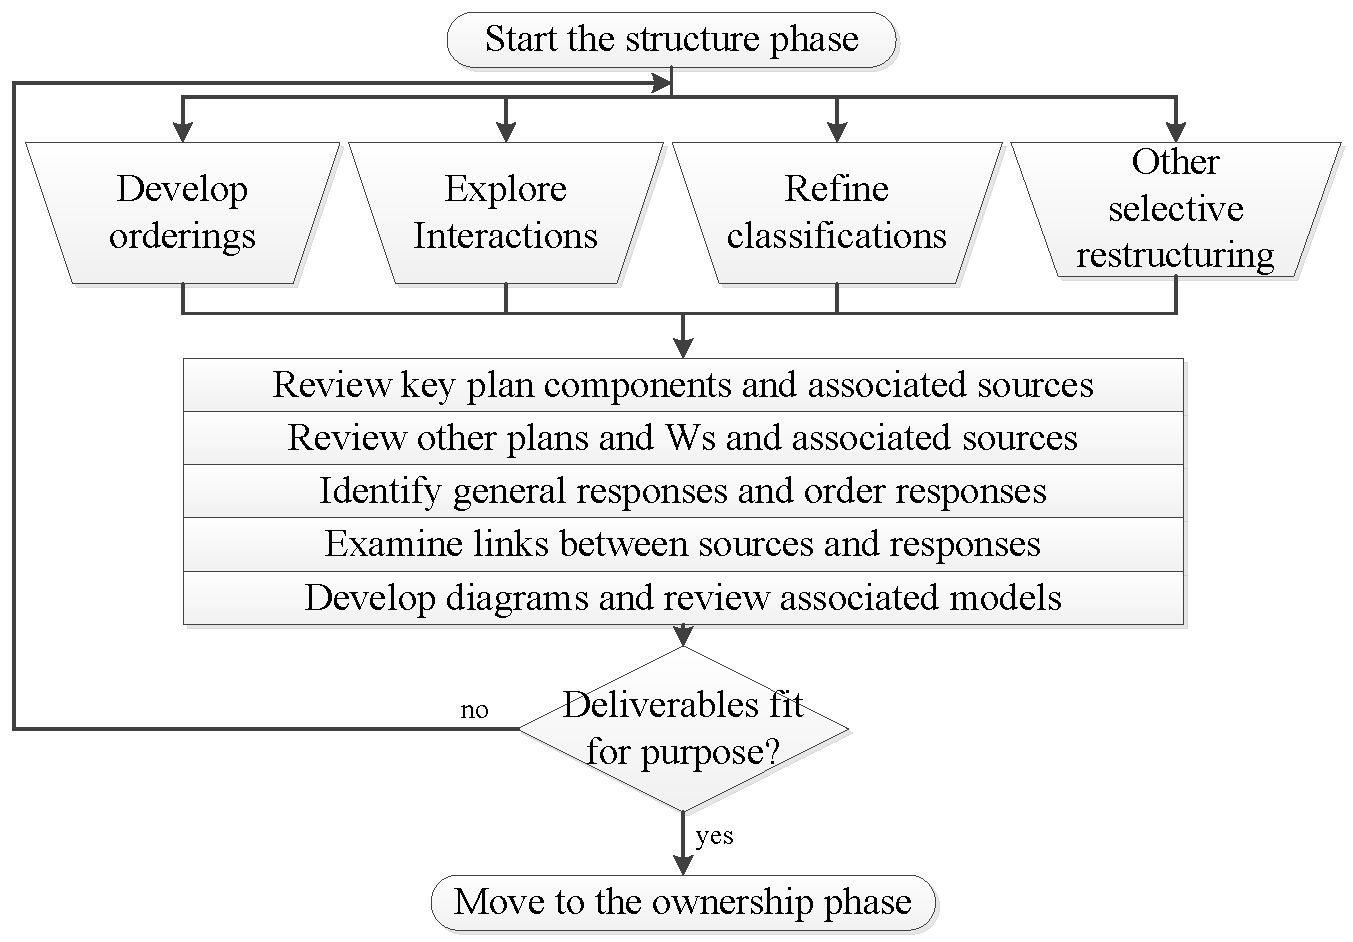
\includegraphics[width = 0.7\textwidth]{./Figures/Structure.png} 
\caption{Structure phase process - adapted from \cite{chapman}}
\label{Figure:Structure}
\end{figure}

The clarify \textbf{ownership} phase allocates financial and managerial responsibility for relevant sources of uncertainty.
In reality, all sources are allocated to a party whether explicitly or by default.
The key activities of this stage include developing a contracting strategy, distinguishing ownership and allocating responsibility.
The aim of the phase is a win-win outcome for all contractual parties, so that client and contractor objectives are aligned.

\begin{figure}[!h]
  \centering
\subfigure[Ownership phase process]{
    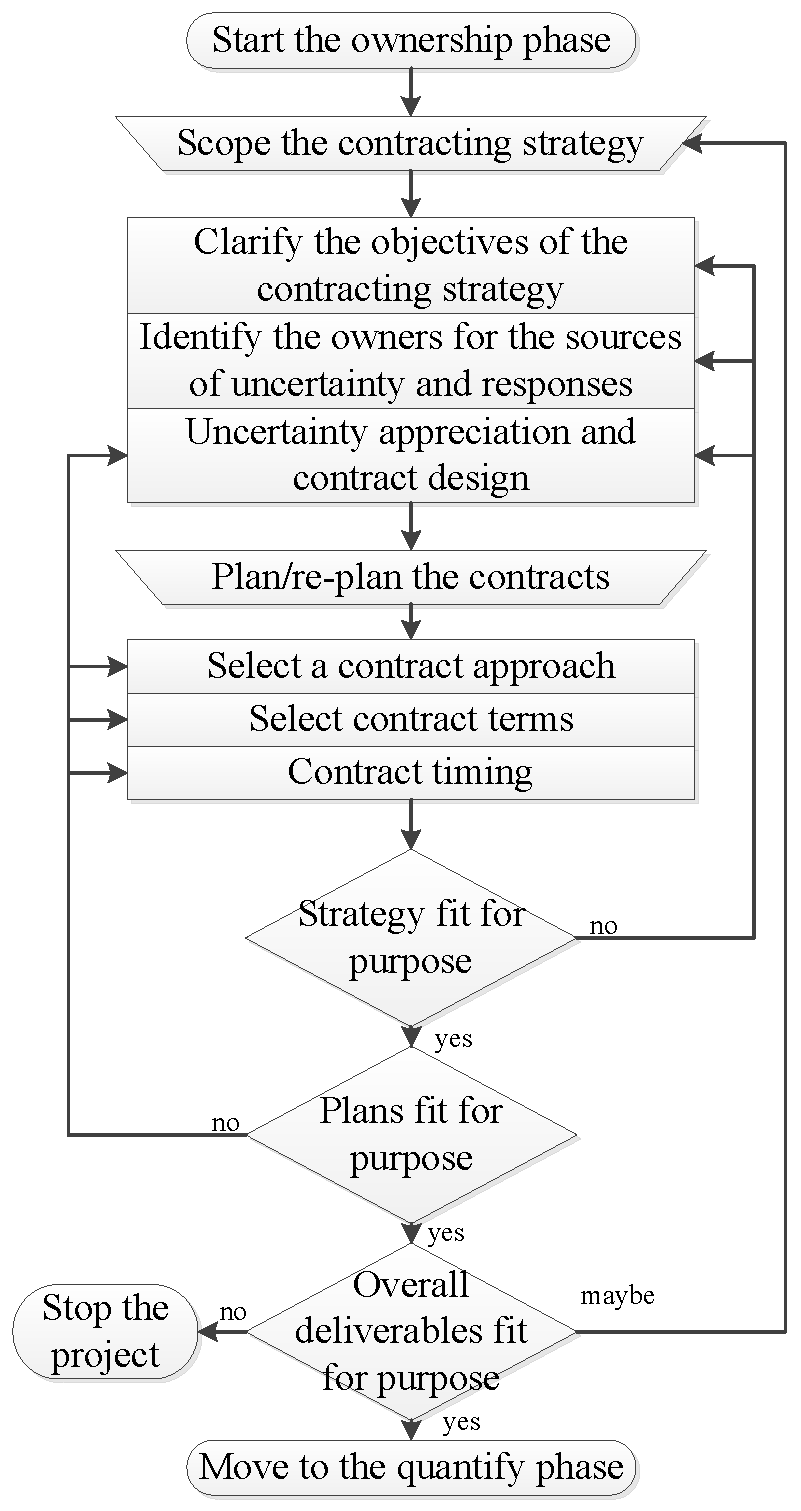
\includegraphics[height = 12cm]{./Figures/Ownership.png} 
	\label{Figure:Owner}
   } \quad
\subfigure[Quantify phase process]{
    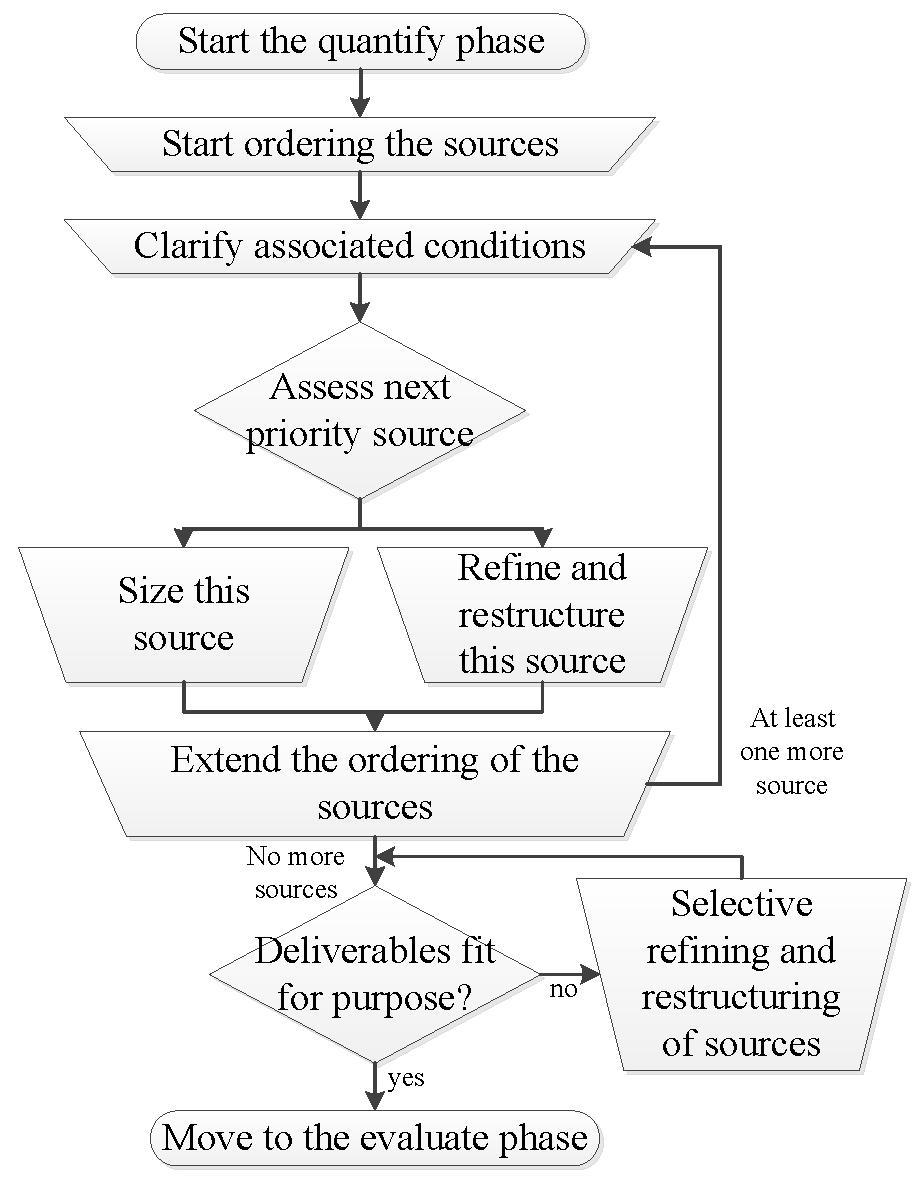
\includegraphics[height = 12cm]{./Figures/Quantify.png} 
	\label{Figure:Quantify}
   }
\caption{Phase process flowcharts - adapted from \cite{chapman}}
\label{Figure:OwnQuant}
\end{figure}

The key deliverable of the \textbf{Quantify} phase is an informed basis for making critical project decisions in the pursuit of opportunity efficiency.
Clarity efficiency is achieved by sizing the data on the first iteration and decomposing to subsequent levels of detail where necessary in further iterations.
Probability impact grid (PIG) approaches are widespread in industry.
PIGs suffer from subjective interpretation of measuring terms \citep{Merkhofer}, a failure to address uncertainty of other than event uncertainty and granular quantisation of sources \citep{Cox2008}.
Where objective data is available, probabilistic density functions should be utilised.
It would be foolish to disregard the expertise of experienced personnel; subjective probabilities provide a method of using this information in the absence of objective data.
The SRI technique published by \citet{spetzer} provides a framework for probability elicitation.
There are some complexities discussed by \citet{Merkhofer}, including strategic misrepresentation \citep{flyvbjerg} and it remains an inexact science.


\begin{figure}[!h]
  \centering
\subfigure[Example 5x5 pig approach - adapted from \cite{Cox2008}]{
    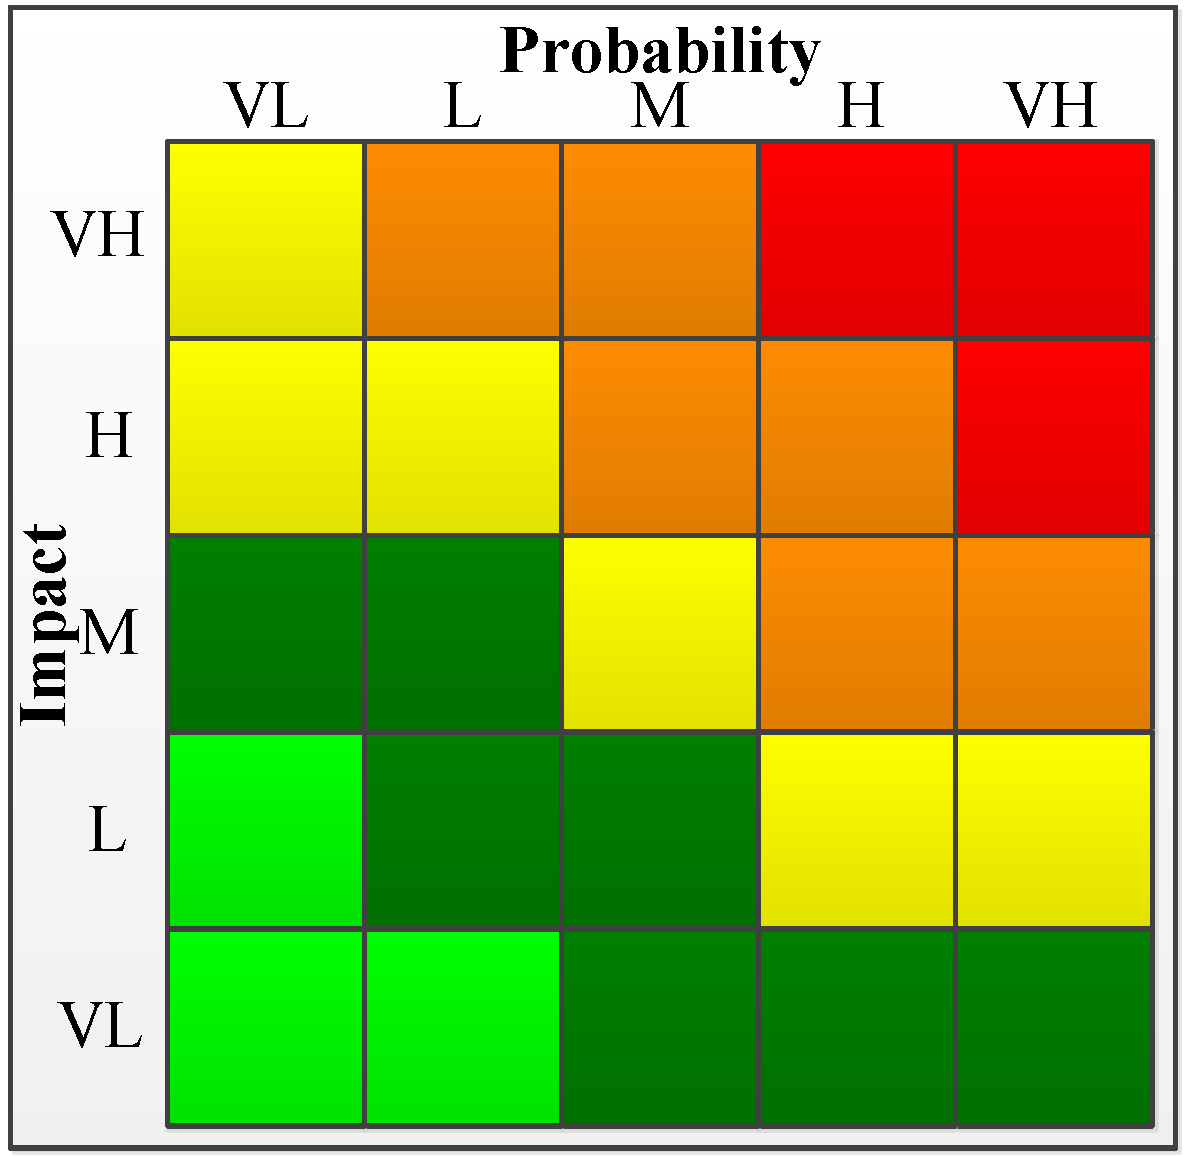
\includegraphics[height = 7cm]{./Figures/PIGCox.png} 
	\label{Figure:PIG}
   } \quad
\subfigure[Example methods for developing probability density functions - adapted from \cite{chapman}]{
    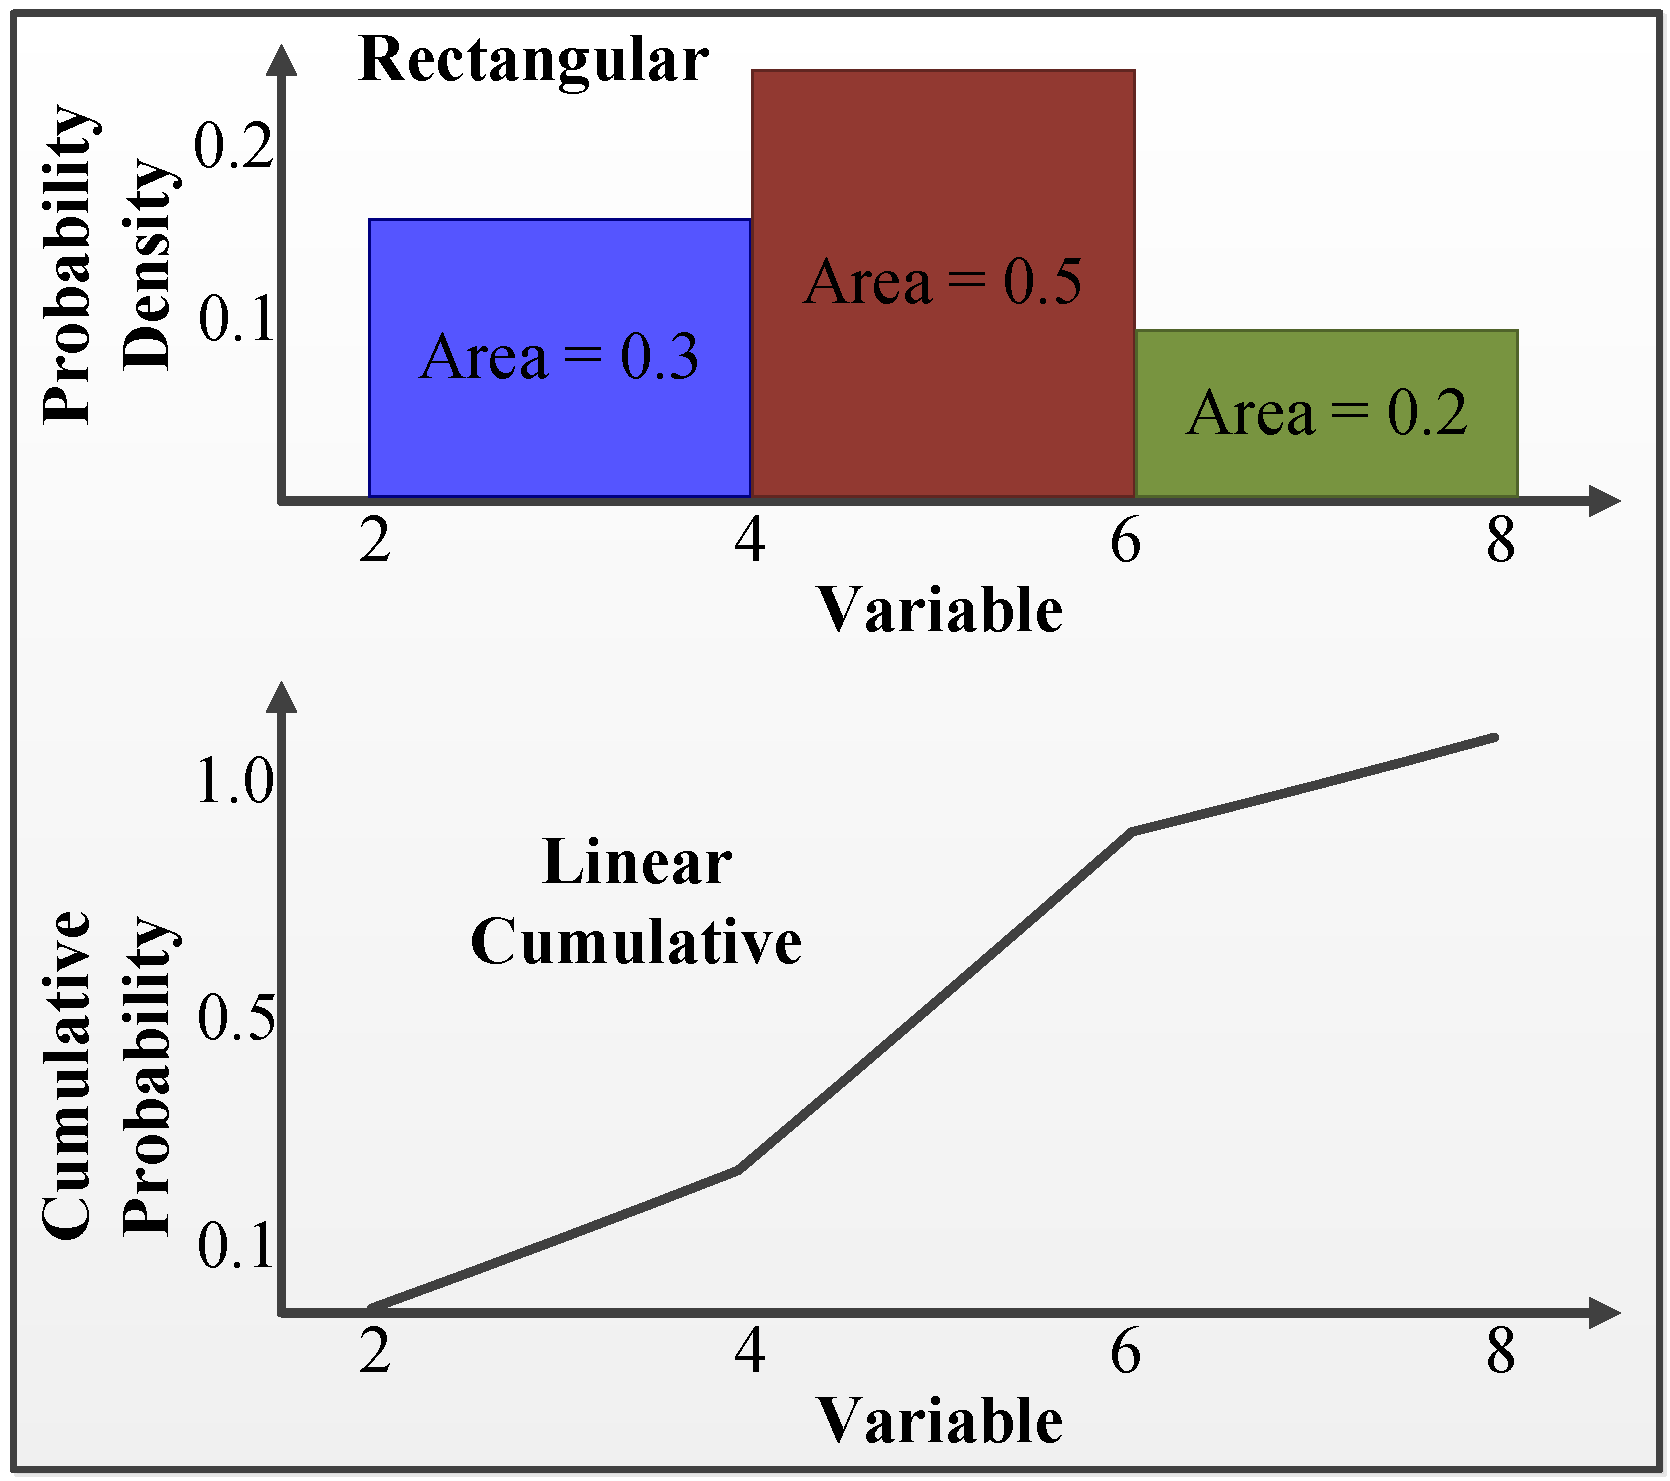
\includegraphics[height = 7cm]{./Figures/Hist.png} 
	\label{Figure:Hist}
   }
\caption{Potential approaches to the quantification of data}
\label{Figure:PIGPDF}
\end{figure}


The \textbf{evaluate} phase involves synthesizing the results of the quantify phase and assessing the statistical significance of results.
This phase is critical to the successful application of the PUMP process, and consolidates much of the understanding of uncertainty.
This phase is considered in detail in section \ref{s:Evaluate}.


\subsection{The Clarity Efficient Approach to Opportunity Efficiency}
This section has given a brief overview of a high clarity PUMP for the E\&D strategy shaping phase, except for the identify and evaluate phases considered later.
Several recurring themes throughout all PUMP phases have been illustrated including the pursuit of clarity efficiency, flexibility and a holistic approach to uncertainty management to achieve opportunity efficiency.
The following sections will consider the Identify and Evaluate phases in detail.


%1200words.